\section{Abstract}

O-C shell mergers in massive stars are a site for the production of the p-nuclei via the $\gamma$-process. 
During these mergers, the ingested C-shell material undergoes convective-reactive nucleosynthesis in the O-burning shell where the timescales for advection and nuclear reactions become equal.
1-D stellar models rely on the predictions of mixing length theory which does not match the results of 3-D hydrodynamic simulations in this region.
In this paper, we use the $M_{\mathrm{ZAMS}}=15 M_\odot$, $Z=0.02$ model from the NuGrid stellar data set \cite{ritterNuGridStellarData2018} to create a detailed post-processed model of the O-shell during a merger event to investigate how 3-D macrophysics impacts nucleosynthesis.
This is done by introducing a convective downturn at the bottom of the O-burning shell, varying the rate of ingesting C-shell material, and implementing a dip in the difussion profile due to both a GOSH-like event and partial merger.
In addition to this, we also investigate the impact of varying the input nuclear physics of all photo-disintegration reactions of unstable p-heavy isotopes from Se$-$Po by a factor of $10$ up and down in a Monte Carlo way in various mixing conditions.
The results show that the mixing details have a significant impact on the production of the p-nuclei and influence the impact of the nuclear physics.
Introducing a convective downturn has a non-linear, non-monotonic impact on the production of the p-nuclei, with an average spread of $0.96~\mathrm{dex}$ between MLT and downturn scenarios.
Increasing the C-shell ingestion rate is found to increase production and has a spread in production of $1.22-1.84~\mathrm{dex}$ across MLT and convective downturn scenarios.
GOSH-like and partial merger dips where were found to decrease production in a uniform way by and hasa  spread in production including MLT of $0.51~\mathrm{dex}$.
Finally, the nuclear physics impact was found to have cause a spread in the final mass fraction on average $0.56-0.79~\mathrm{dex}$ across mixing scenarios which is similar to the spread across the various mixing scenarios.
Additionally, we find whether there is a correlation and the strength of it are both dependent on the mixing scenario.
We conclude that understanding the mixing details of the O-C shell merger along with the nuclear physics is critical for understanding the production of p-nuclei and that there are comparable model uncertainties as the nuclear physics.

\section{Introduction} \label{sec:intro}

The question of how to replicate the solar pattern of the 35 stable ``p-nuclei''
\footnote{They are $^{74}\mathrm{Se}$,$^{78}\mathrm{Kr}$,$^{84}\mathrm{Sr}$,$^{92}\mathrm{Mo}$,$^{94}\mathrm{Mo}$,$^{96}\mathrm{Ru}$,$^{98}\mathrm{Ru}$,$^{102}\mathrm{Pd}$,$^{106}\mathrm{Cd}$,$^{108}\mathrm{Cd}$,$^{113}\mathrm{In}$,$^{112}\mathrm{Sn}$,$^{113}\mathrm{Sn}$,$^{115}\mathrm{Sn}$,$^{120}\mathrm{Te}$,$^{124}\mathrm{Xe}$,\linebreak$^{126}\mathrm{Xe}$,$^{130}\mathrm{Ba}$,$^{132}\mathrm{Ba}$,$^{138}\mathrm{La}$,$^{136}\mathrm{Ce}$,$^{138}\mathrm{Ce}$,$^{144}\mathrm{Sm}$,$^{152}\mathrm{Gd}$,$^{156}\mathrm{Dy}$,$^{158}\mathrm{Dy}$,$^{162}\mathrm{Er}$,$^{164}\mathrm{Er}$,$^{168}\mathrm{Yb}$,$^{174}\mathrm{Hf}$,$^{180\mathrm{m}}\mathrm{Ta}$,$^{180}\mathrm{W}$,$^{184}\mathrm{Os}$,\linebreak$^{190}\mathrm{Pt}$,$^{196}\mathrm{Hg}$}
 has been a long-standing problem in nucleosynthesis.
 It was originally considered that these isotopes had no contribution from the $s$- and $r$-processes, and it was proposed by \cite{burbidgeSynthesisElementsStars1957} that they were created via $(p,\gamma)$, $(n,\gamma)$, and $(\gamma,n)$ reactions in Type II supernovae (SNe) in a process called the $p$-process.
A variety of processes and astrophysical sites have been discussed as a site for the production of the p-nuclei, but there is not a single site for the production of them all.
\cite{woosleyAlphaProcessRProcess1992} found that the $\alpha$-rich freezeout in supernova can produce $^{74}\mathrm{Se}-$$^{92}\mathrm{Mo}$. 
\cite{frohlichNeutrinoInducedNucleosynthesisA>642006} and \cite{arconesProductionLightelementPrimary2011} both found that high neutrino fluxes during a supernova can create a proton rich environment in a process called the $\nu p$-process that produce $^{74}\mathrm{Se}-$$^{108}\mathrm{Cd}$.
\cite{schatzRpprocessNucleosynthesisExtreme1998} suggest that a hydrogen-rich accretion disk around a neutron star could undergo a series of rapid proton captures called the $rp$-process that produce $^{74}\mathrm{Se}-$$^{98}\mathrm{Ru}$.
\cite{xiongProduction$p$Nuclei2024} propose that neutrino induced reactions of $r$-process material in a $\nu r$-process could produce the p-nuclei from $^{78}\mathrm{Kr}-$$^{138}\mathrm{La}$ and argue that these conditions could be met in the winds of a proto-neutron star. 
\cite{gorielyHedetonationSubChandrasekharCO2002} propose that a proton-poor but neutron boosted region could undergo proton-captures similar to the $rp$-process but can extend to the heavier p-nuclei as well as the light in a process called the $pn$-process during He-detonation of a C-O white dwarf's ejected envelope.
\cite{travaglioTypeIaSupernovae2011} found that they could produce p-nuclei via the photo-disintegration of $s$-process material via the $\gamma$-process in SNIa could produce the not only the p-nuclei, but also the notoriously underproduced isotopes $^{92,94}\mathrm{Mo}$ and $^{96,98}\mathrm{Ru}$. 
In a follow-up paper, \cite{travaglioTestingRoleSNe2015} found that the s-process distribution of seed material for the $\gamma$-process was very signifcant on the production of p-nuclei in this scenario, especially the heaviest ones, and that there is a heavy metallicity dependency on the lightest three p-nuclei.
\cite{battinoHeavyElementsNucleosynthesis2020} found that rapidly accreting white dwarfs that have H-flashes achieve neutron densities necessary for the $i$-process that modify the seed distribution so that it could produce the p-nuclei in the range $96 < A < 196$ during the subsequent SNIa.
In massive stars, \cite{pignatariProductionProtonrichIsotopes2016} argue that the weak $s$-process can modify the seeds before the CCSN to boost production of the p-nuclei via the $\gamma$-process during the explosion.

There is contention whether all of the classical 35 isotopes are ``p-nuclei''.
\cite{bisterzoSprocessLowmetallicityStars2011} found that $^{152}\mathrm{Gd}$, $^{164}\mathrm{Er}$, and $^{180}\mathrm{Ta}$ have $70.5\%$, $75.5\%$, and $74.5\%$ respectively have $s$-process contribution.
\cite{dillmannPProcessSimulationsModified2008} argues that $^{113}\mathrm{In}$ and $^{115}\mathrm{Sn}$ are made in $\beta$-decays post $r$-process via isomeric states.
\cite{gorielyPuzzleSynthesisRare2001} found that $(\gamma,n)$ was too weak to produce $^{138}\mathrm{La}$, and instead that it is made by $\nu_e$-capture on $^{138}\mathrm{Ba}$ during the explosion of a $M_{\mathrm{ZAMS}}=25M_\odot$ star.
\cite{arnouldPprocessStellarNucleosynthesis2003} say that it is possible that $^{180\mathrm{m}}\mathrm{Ta}$ could have contributions from $\nu$-induced nucleosynthesis similar to $^{138}\mathrm{La}$.
\cite{sieverdingNProcessLightImproved2018} also found that the $\nu$-process is important for $^{113}\mathrm{In}$, $^{138}\mathrm{La}$, and $^{180}\mathrm{Ta}$.

In this paper, we will be focused on how the $\gamma$-process in massive stars pre-supernova produce the p-nuclei.
The $\gamma$-process describes the flow of $(\gamma,n)$, $(\gamma,p)$, and $(\gamma,\alpha)$ reactions on the stable $s$-, $i$-, and $r$-process seeds that are already present \cite{rauscherConstrainingAstrophysicalOrigin2013}.
\cite{arnouldPossibilitySynthesisProtonrich1976} argue that hydrostatic O-burning at temperatures of $2 \mathrm{~GK}$ could be a site for the production of p-nuclei, and \cite{woosleyPprocessesSupernovae1978} continued to describe the production of p-nuclei by photo-disintegrating the heavy elements at temperatures of $2-3\mathrm{~GK}$ during explosive carbon and oxygen burning. 
\cite{rauscherNucleosynthesisMassiveStars2002} found in their $M_{\mathrm{ZAMS}}=20 M_\odot$ massive star model had pre-explosive production of the p-nuclei during a merger of the convective oxygen, carbon, neon shells right shortly before the model underwent a core collapse supernova (CCSN).
\cite{rauscherConstrainingAstrophysicalOrigin2013} say that the effective temperature range for producing the p-nuclei by the $\gamma$-process and the $\nu p$-process is $1.5\leq T \leq 3 \mathrm{~GK}$.
Although the $\gamma$-process can produce across the mass range, there are known problems with this process.
\cite{woosleyNucleosynthesisRemnantsMassive2007} found that the $\gamma$-process in the supernova of massive stars was deficient for those between $A=90-130$ and 
\cite{arnouldPprocessStellarNucleosynthesis2003} note that particularly $^{92,94}\mathrm{Mo}$ and $^{96,98}\mathrm{Ru}$ are underproduced by the $\gamma$-process in CCSN. 
Further, \cite{rayetPprocessRevisited1990} and \cite{dillmannPProcessSimulationsModified2008} argue that $^{113}\mathrm{In}$, $^{115}\mathrm{Sn}$, $^{152}\mathrm{Gd}$, $^{164}\mathrm{Er}$ and $^{180\mathrm{m}}\mathrm{Ta}$ are weakly produced or even destroyed during the $\gamma$-process and should not even be considered as p-nuclei.

\cite{robertiGprocessNucleosynthesisCorecollapse2023} looked at two massive star models with O-C shell mergers and found that most of the p-nuclei with $A > 110$ were dominantly produced during the merger and not from explosive CCSN nucleosynthesis. 
These stellar models were the $M_{\mathrm{ZAMS}}=15 M_\odot$ $Z=0.02$ from \cite{ritterNuGridStellarData2018} and $M_{\mathrm{ZAMS}}=20 M_\odot$ $Z=0.02$ model from \cite{rauscherNucleosynthesisMassiveStars2002}.
\cite{robertiGprocessNucleosynthesisCorecollapse2024b} found this result to be independent of the peak energy of the CCSN. 
This is a concern because the mixing details of how the material moves in these 1-D stellar models are described by mixing length theory (MLT) which is a time-averaged theory over a pressure scale height. 
\cite{bazanConvectionNucleosynthesisCore1994} found in their 2D simulation of convective O-burning that the region was not accurately described by MLT and was spherically asymmetric. 
They also speculate that the details of nucleosynthesis would be affected by this, which was confirmed in the 3-D simulations of a O-C merger by \cite{rizzutiShellMergersLate2024a}.
The way that mergers occur in \cite{rizzutiShellMergersLate2024a} is also signifcantly different to how it occurs in 1-D.
In their 1-D model, just as in \cite{ritterNuGridStellarData2018}, the upper boundary of the convective O-shell grows in extent, but in their 3-D merger models the bottom boundary of the convective C-shell extends down and subsumes the convective Ne- and O-burning shells.
This underscores how different the macrophysics in 3-D can be compared to 1-D.
\cite{herwigCONVECTIVEREACTIVEPROTON2011} also found that MLT does not accurately describe how mixing occurs in convective-reactive environments. 
Additionally, in their 3-D O-shell burning simulation, \cite{jonesIdealizedHydrodynamicSimulations2017} found that MLT both underestimates the convective velocities and the qualitative shape of those velocities when compared to the 3-D radially averaged velocities. 
\cite{andrassy3DHydrodynamicSimulations2020} found in their 3-D O-C shell mergers that the merger had large-scale non-radial asymmetries that significantly deviated from the spherically symmetric scenario. 
These asymmetries are also seen in the 3-D O-Ne shell merger simulations of \cite{yadavLargescaleMixingViolent2020a}.
\cite{collinsPropertiesConvectiveOxygen2018} also argue that MLT does not accurately describe the convective shell burning velocities as well as both the properites of the shell mergers and how it responds to nuclear burning.
They also identify that the O-burning shell in the O-C shell merger would not be well-mixed as the C-shell material burns as it mixed downwards.
This is a marker of this being a convective-reactive environment as seen in \cite{ritterConvectivereactiveNucleosynthesisSc2018}.
It is clear that a 1-D spherically symmetric MLT is inadequate to describe the mixing details of the O-C shell merger.
Since the O-C shell merger dominates the production of many of the p-nuclei and the mixing details of the O-shell are not well understood in 1-D, the nucleosynthesis is left an open question.

To address the insufficiencies in MLT, we present in this paper a 3D-hydrodynamic inspired approach to 1-D modelling to determine the impact of the mixing on the nucleosynthesis of the $\gamma$-process in the O-shell as C-shell material is entrained. 
By incorporating the insights from 3-D O-shell burning and O-C shell merger simulations, the impact on nucleosynthesis related to the mixing details in 1-D can be demonstrated. 
In addition to this, the impact of nuclear physics in this situation will also be explored.
In Section \ref{sec:methods} we present the methods of how the \cite{ritterNuGridStellarData2018} model is post-processed, how the 3-D hydrodynamic results are incorporated, and how the nuclear physics impact is determined. 
In Section \ref{sec:convreacflow} we explore the nucleosynthesis pathways of $\gamma$-process in this convective-reactive environment. 
Next, in Sections \ref{sec:convdownturnimpact}-\ref{sec:goshimpact} we explore how different mixing details can impact the production of the p-nuclei. 
Section \ref{sec:convdownturnimpact} explores the introduction of a convective downturn at the bottom of the O-shell, Section \ref{sec:ingestionimpact} explores how the ingestion rate impacts the production, and Section \ref{sec:goshimpact} explores the impact from both a GOSH-like event and partial merger.
Then in Section \ref{sec:nuclearimpact} the impact from the nuclear physics and its relationship to the mixing details is explored. 
We will not be considering how modification of the initial seed composition in the C-shell or metallicity, how other models with O-C shell mergers are affected by changes to the mixing, providing nuclear physics uncertainties, investigating the effects of rotation, nor continuing stellar evolution and subsequent CCSN of the model.
Additionally, we will only consider how the O-shell behaves under these conditions and not include the C-shell in the post-processing as the material will only be mixed up higher and no longer undergo the $\gamma$-process because it will be too cold.
This O-shell post-processing will be static with a constant ingestion rate as stellar evolution with dynamic effects like energy feedback will not be calculated.
  
\section{Methodology} \label{sec:methods}

In this paper we post-process the massive stellar model $M_{\mathrm{ZAMS}}=15 M_\odot$,  $Z=0.02$ in the NuGrid data set \citep{ritterNuGridStellarData2018}.
This model has a merger of its convective O and C-burning shells late in its evolution as shown in Figure \ref{fig:kippenhahn}.
During this merger, the C-burning ashes and $s$-process material are ingested into the much hotter O-burning shell.

\begin{figure}[!htbp]
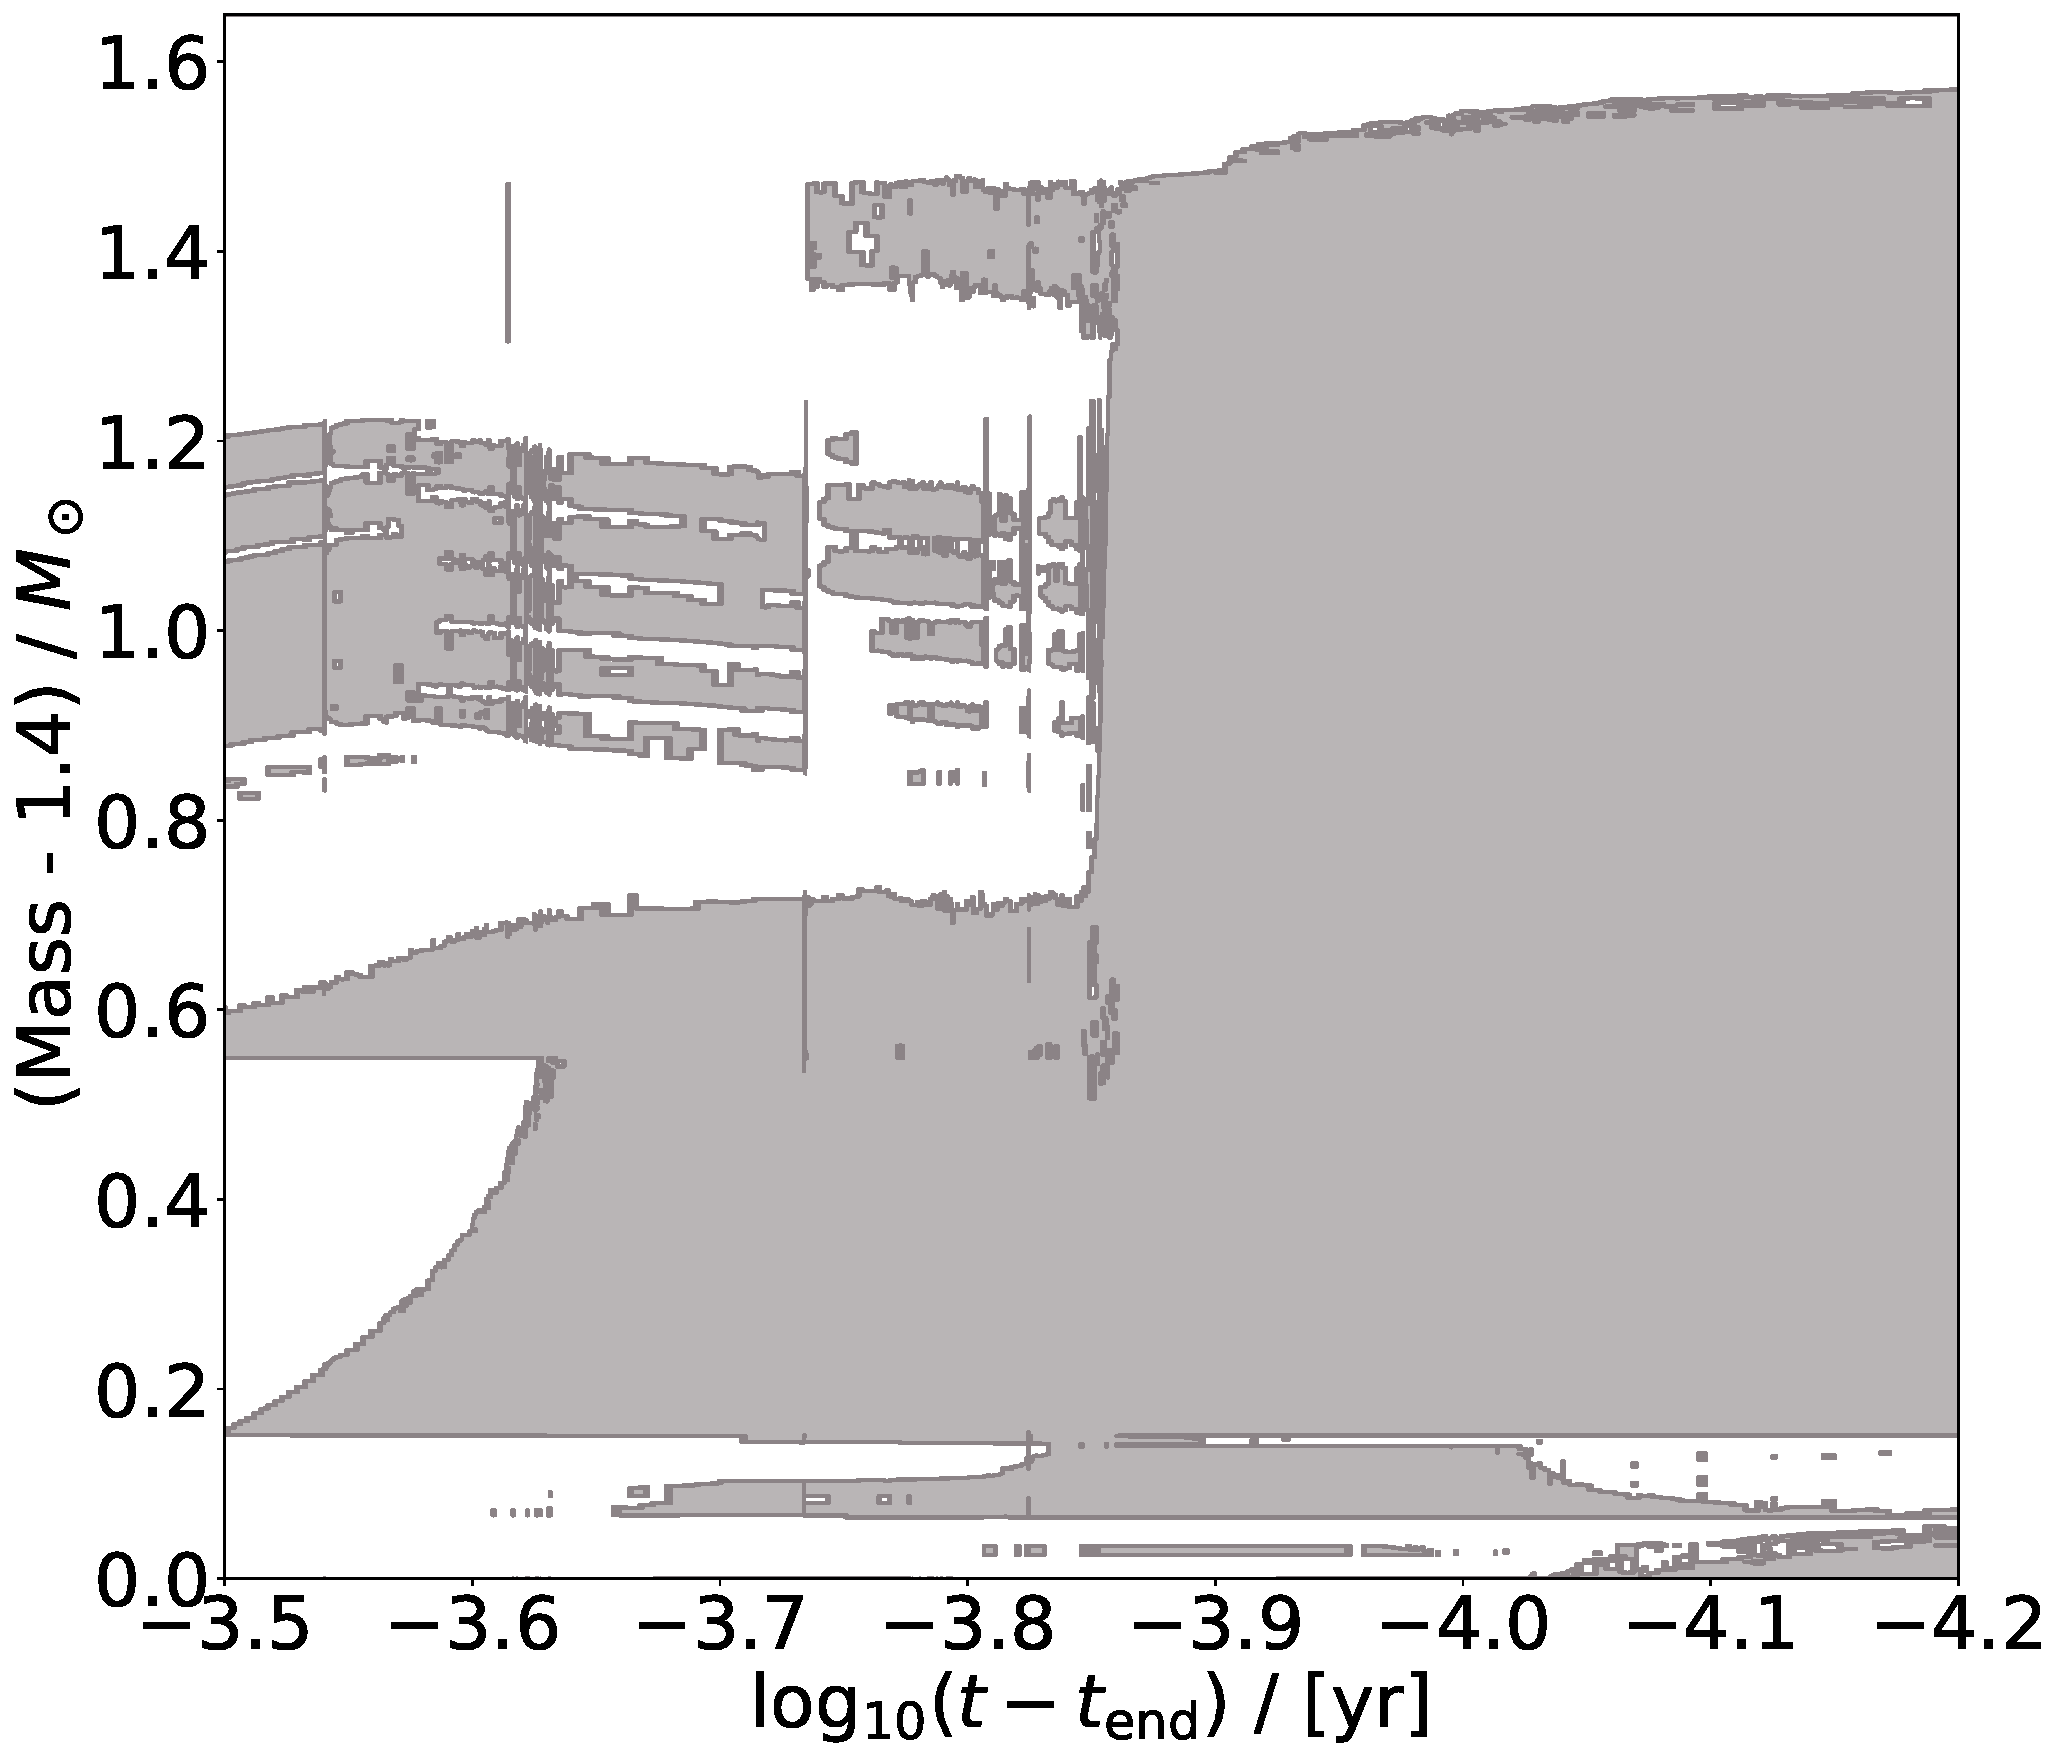
\includegraphics[width=\textwidth]{chapters/2/figures/Kippenhahn_Ritter+2018.pdf}
\caption{Kippenhahn diagram showing the merger of the convective O and C-burning shells. The O-burning shell extends from $1.55 M_\odot$ to $1.95 M_\odot$. The first convective C-burning shell sits directly on top from $1.96 M_\odot$ to $2.11 M_\odot$ and additional convective C-burning shells that are subsumed are above. The merger onsets at $\log_{10}(t-t_{\mathrm{end}}) /\mathrm{yr} \approx -3.85$ and reaches full extent at $\approx-4$.
\label{fig:kippenhahn}}
\end{figure}

The detailed nucleosynthesis is calculated with the 1-D multi-zone post-processing code \texttt{MPPNP} using a nuclear network of 1470 isotopes to post-process only the O-shell.
\texttt{MPPNP} does not include isomeric states in its network, so the nucleosynthesis of the p-nuclei $^{180\mathrm{m}}\mathrm{Ta}$ is not calculated although we calculate the production of the ground state $^{180}\mathrm{Ta}$. 
In addition to calculating the nucleosynthesis for each timestep, the species in the O-shell is also decayed at a temperature of $T=100~\mathrm{MK}$ without contributions from explosive nucleosynthesis.
The results of this work are presented in terms of an overproduction compared to the solar measurement $\mathrm{OP}$ given by the equation
$$\mathrm{OP} = \log_{10}\Biggl(\frac{X_{i}}{X_{i,\odot}}\Biggr)$$
where $X_{i}$ is the final decayed mass fraction of a species in the O-shell and $X_{i,\odot}$ is the solar measurement of the species from \cite{grevesseAtomicDataSolar1994}.

A static stellar structure is taken from the onset of the merger at $\log_{10}(t-t_{\mathrm{end}}) /\mathrm{yr}=-3.856$ and an initial isotopic composition from right before onset of merger $\log_{10}(t-t_{\mathrm{end}}) /\mathrm{yr}=-3.845$.
As such, we calculate C-shell ingestion for $110 \mathrm{~seconds}$ with a constant ingestion rate of $4\times10^{-3} M_\odot\mathrm{s^{-1}}$ for all models except those in Section \ref{sec:ingestionimpact}. 
This rate is the mass of the O-shell divided by the ingestion time.
To determine the behavior during the merger, the diffusion coefficient profile is forced into a merged state as seen in Figure \ref{fig:dmlt_forced}. 

\begin{figure}[!htbp]
\includegraphics[width=\textwidth]{chapters/2/figures/Dmlt_forced.pdf}
\caption{The diffusion coefficient profile predicted by MLT at model number 9160 for the $M_{\mathrm{ZAMS}}=15 M_\odot$, $Z=0.02$ model and the forced merger profile for the O-shell. The red line with triangles is the MLT prediction and the blue line is the forced merger. The black lines are the boundaries of the convective O-burning shell. 
\label{fig:dmlt_forced}}
\end{figure}

\subsection{1-D implementation of 3-D macrophysics}\label{sec:mixing_methods}

Since the predictive power of MLT on the mixing is insufficient, we incorporate insights from 3D-hydrodynamic simulations into our 1-D models. 
In their 3-D convective O-burning simulation \cite{jonesIdealizedHydrodynamicSimulations2017} found that a convective profile downturn is present in the 3-D radially averaged convective velocity profile that is not found in MLT.
That means that MLT predictions cannot describe behaviour in this region at all.
MLT also underpredicts the strength of the convective velocities in this region.
\cite{jonesIdealizedHydrodynamicSimulations2017} found that convective velocities are stronger by a factor of $\sim 30$ when compared to the MLT predictions. 
\cite{andrassy3DHydrodynamicSimulations2020} in their 3-D C-shell entrainment simulations that their velocities could be a factor of $\sim 5$ stronger depending on the strength of carbon and oxygen burning, and \cite{rizzutiShellMergersLate2024a} a boost of $\sim 10$ due to the feedback of new reactions from the ingested material in their 3-D O-C shell mergers. 
The downturn in the profile is incorporated in this work using the recommendation from \cite{jonesIdealizedHydrodynamicSimulations2017}:
\begin{equation}
    D_{\mathrm{3D-insp.}} = \frac{1}{3} v_{\mathrm{MLT}}\times\min{(\ell,r-r_0)}
\end{equation} 
where $\ell$ is the mixing length and $r_0$ is the Schwarzschild boundary at the bottom of the O-shell and an increasingly strong boost factor is applied of $3\times$, $10\times$, and $50\times$ to the convective velocities as shown in Figure \ref{fig:all_dconv} to match what is seen in the 3-D simulations.

The $50\times$ boost factor is higher than what is seen in these simulations, but it is possible that they underestimate the boost in convective velocities from the feedback of ingested material reacting in the O-shell since they have limited nuclear networks.
Although \cite{jonesIdealizedHydrodynamicSimulations2017} considers the downturn at the top of the O-shell, it is adopted at the bottom of this shell as it is understood to be merged with the C-shell on top.
This is justified by the simulations done by \cite{meakinTurbulentConvectionStellar2007} who show a downturn at both the bottom and top of their 2-D and 3-D O-shell burning simulations.
Another insight from 3-D models is that the entrainment rate of the C-shell could vary \citep{andrassy3DHydrodynamicSimulations2020}. 
To investigate how this impacts the p-nuclei, a rate of $4\times10^{-5}M_\odot~\mathrm{s^{-1}}$ and $4\times10^{-4}M_\odot~\mathrm{s^{-1}}$ are also calculated along with our default rate of $4\times10^{-3}M_\odot~\mathrm{s^{-1}}$ for the MLT and all 3D-inspired mixing scenarios. 
In addition to this, a scenario is considered for all mixing scenarios where there is no ingestion of C-shell material.

\begin{figure}[!htbp]
\includegraphics[width=\textwidth]{chapters/2/figures/All_Dconv.pdf}
\caption{The diffusion coefficient profiles for the 3D-inspired mixing scenarios. The blue dashed line is the merged $D_{\mathrm{MLT}}$ profile,  the orange line with diamonds, green line with triangles, red line with red circles, and purple line with squares are those calculated using $D_{\mathrm{3D-insp.}}$ with boost factors of $1$, $3$, $10$, and $50$ respectively. 
\label{fig:all_dconv}}
\end{figure}

There are other potential effects that can be considered during this merger.
As there is energy feedback from the ingested C-shell material, this could cause a split in the convective profile as seen in \cite{herwigCONVECTIVEREACTIVEPROTON2011}.
\cite{herwigGLOBALNONSPHERICALOSCILLATIONS2014} found this effect could happen during the ingestion of H into a He-shell in their 3D simulations and labelled this effect Global Oscillation of Shell H-ingestion (GOSH).
It could be that the energy feedback from the ingested C-shell material could have a similar effect to a GOSH.
\cite{andrassy3DHydrodynamicSimulations2020} found that strong oscillatory modes were present in their 3-D simulations of C-shell entrainment into an O-shell.
Another potential effect is that the convective profiles of the O-shell and C-shell do not fully merge. 
To determine the impact on nucleosynthesis in both a GOSH-like and partial merger event, both scenarios are tested at two different strengths each.
Using
\begin{equation}
D_{\mathrm{dip}}=D_{\mathrm{MLT}}-(D_{\mathrm{MLT}}-c)\times\exp\Biggl[-\frac{(r-a)^2}{w^2}\Biggr]
\end{equation}
a dip is put into the diffusion coefficient profile $D_{\mathrm{conv}}$ where $c$ is the minimum value of the dip, $w$ the width, and $a$ the center. 
For all four scenarios have a width $w=0.25~\mathrm{Mm}$, the weaker of the scenarios the dip descends to $c=10^{14}~\mathrm{cm^2s^{-1}}$ and the stronger $c=10^{13}~\mathrm{cm^2s^{-1}}$.
The GOSH-like scenarios are centered at $a=4.95~\mathrm{Mm}$ where $D_\alpha=1$ for $^{20}\mathrm{Ne}(\gamma,\alpha)$$^{16}\mathrm{O}$ which could be one of the sources for this energy feedback at peak $^{20}\mathrm{Ne}$ burning.
The partial merger scenarios are centered at $r=7.5\mathrm{~Mm}$ where the unmerged $D_{\mathrm{MLT}}$ has a dip as seen in Figure \ref{fig:dmlt_forced}. 
The profiles for the GOSH-like and partial merger scenarios are shown in Figure \ref{fig:dgosh_partial}.

\begin{figure}[!htbp]
\includegraphics[width=\textwidth]{chapters/2/figures/Dmlt_partial_gosh.pdf}
\caption{The MLT, GOSH-like, and partial merger diffusion coefficient profiles. The blue dashed line is $D_{\mathrm{MLT}}$, the pink line with triangles and lime line are potential GOSH-like splits in the profile centered at $r=4.95~\mathrm{Mm}$, the purple line has a dip that is $10\times$ deeper. The brown line with circles and the turquoise line are partial mergers $r=7.5~\mathrm{Mm}$, the gray line has a dip that is $10\times$ deeper. The black dashed lines are the edges of the O-shell.
\label{fig:dgosh_partial}}
\end{figure}

\subsection{Determining nuclear physics impact}\label{sec:nuclear_methods}

There are many unmeasured reaction rates for the unstable proton heavy isotopes from $\mathrm{Se}-\mathrm{Po}$ which means that there is are possible variation in the input nuclear physics of the $\gamma$-process. 
To determine the impact of varying the nuclear physics in this region, the photo-disintegration rates $(\gamma, \alpha)$, $(\gamma, p)$, $(\gamma, n)$ for all unstable proton heavy isotopes from  $\mathrm{Se}-\mathrm{Po}$ are varied in our network along with their corresponding capture rates by a random factor between 0.1 to 10 that is uniformly selected in a Monte Carlo (MC) way for 1000 scenarios.
This extends the approach performed by \cite{denissenkovImpactReactionRate2018} and \cite{denissenkovImpactNgReaction2021} for $(n, \gamma)$ rates in an i-process context. 
This was done for the MLT mixing scenario and the four 3D-inspired mixing scenarios but not the GOSH-like and partial merger scenarios.
This approach also allows for the identification of reaction rates that are relevant for the production of an isotope using correlations.
The Pearson coefficient describes correlations between $X/X_{\mathrm{no~variation}}$ and the variation factors where $X$ is the final decayed mass fraction of a Monte Carlo case and $X_{\mathrm{no~variation}}$ is the final decayed mass fraction for the default case where all varation factors are equal to $1$.
All correlations $|r_\mathrm{P}| \geq 0.15$ are reported in this study.
In addition to the Pearson coefficient, a logarithmic slope $\zeta$ is also reported to determine the importance of a reaction on the final mass fraction of an isotope.
The importance of considering $\zeta$ as well as additional caveats for the correlated rates are discussed in Section \ref{sec:appendixNuclearRates}.

\section{Correlations of nuclear reaction rates}\label{sec:appendixNuclearRates}

The Pearson correlation coefficient, $r_\mathrm{P}$, is insufficient to quantify the importnace of a correlated rate as demonstrated by Figure \ref{fig:corr_ex}.
A strong correlation does not correspond directly to a signifcant change to the final mass fraction of a species.
In addition to the correlation coefficient, a slope $\zeta$ is provided that better describes this behaviour.
$\zeta$ is the slope of a linear regression between $\log_{10}(X/X_\mathrm{no~variation})$ and $\log_{10}(\mathrm{variation~factor})$ where $X$ is the final decayed mass fraction for Monte Carlo rates and $X_\mathrm{no~variation})$ is the final decayed mass fraction for the default case where all variation factors are equal to $1$.


\begin{figure}[!htbp]
\includegraphics[width=\textwidth]{chapters/2/figures/correlation_example.pdf}
\caption{Examples of strongly correlated mass fractions with reaction rates for four species for the MLT mixing scenario. The blue dots are the values and the red line is the best linear fit to $\mathrm{OP}_{\mathrm{var}}$ and $\log_{10}(\mathrm{variation~factor})$. The top left plot and bottom right plot show strong correlations for $^{74}\mathrm{Se}$ and $^{196}\mathrm{Hg}$ that directly impact the mass fraction. The top right plot shows a correlation for $^{98}\mathrm{Ru}$ where there is considerable spread in the mass fraction. The bottom left plot shows a correlation for $^{184}\mathrm{Os}$ where the mass fraction is strongly affected only for multiplication factors less than $1$. 
\label{fig:corr_ex}}
\end{figure}

It is clear from Figure \ref{fig:corr_ex} that similarly correlations do not directly mean that the reaction rate is relevant for the production of a species, but the slope $\zeta$ also does not directly point to this.
The bottom right plot showing the impact on the final mass fraction of $^{196}\mathrm{Hg}$ from varying the input rate for $^{196}\mathrm{Pb}(\gamma,n)$ has both a strong slope and correlation, but the bottom left plot has a strong correlation and a weak slope.
Reaction rates that are both highly correlated and have a strong slope will have direct impact on the production of species.

Another caveat is that this method of varying the reaction rates in a Monte Carlo way does not distinguish between the photo-disintegration and corresponding capture rate.
All correlated rates are reported according to their photo-disintegration rates, but as shown by the upper left plot of Figure \ref{fig:corr_ex} for $^{74}\mathrm{Se}$ and $^{75}\mathrm{Se}(\gamma,n)$$^{74}\mathrm{Se}$ this results sometimes in saying that a reaction that would be considered a production term is strongly anti-correlated with production.
This is because when we apply the variation factor, we do so for both $^{75}\mathrm{Se}(\gamma,n)$ and $^{74}\mathrm{Se}(n,\gamma)$.
As Figure \ref{fig:se74_example} shows, both of these reactions have relevant nucleosynthetic fluxes contributing to the final mass fraction of $^{74}\mathrm{Se}$.

\begin{figure}[!htbp]
\includegraphics[width=\textwidth]{chapters/2/figures/Se74_example.pdf}
\caption{Nucleosynthetic flux and mass fraction plot for the MLT mixing case at $t=110~\mathrm{sec}$. The blue solid line and brown dashed line are $^{75}\mathrm{Se}(\gamma,n)$$^{74}\mathrm{Se}$ and $^{74}\mathrm{Se}(n,\gamma)$$^{75}\mathrm{Se}$ respectively. The red solid line with triangles and black solid line with circles are the mass fractions of $^{74}\mathrm{Se}$ and $^{75}\mathrm{Se}$ respectively.
\label{fig:se74_example}}
\end{figure}

This is not the case for all reactions as temperatures can be high enough that the capture rates are potentially not relevant, but as shown in Section \ref{sec:convreacflow} this is an environment where species are co-producing each other and it could be the case.
